\chapter{無線センサネットワークにおけるオペレーティングシステム}\label{chap:os_in_WSN}
\begin{large}
\begin{quote}
本章では,まず,
無線センサネットワークにおけるオペレーティングシステムについての
導入を行う.
次いで,無線センサネットワークにおけるオペレーティングシステムを分類し,
それぞれについて具体的なオペレーティングシステムを例に挙げながら,
その特徴についての考察を行う.
最後に,それぞれのモデルを比較し,
それぞれのモデルを採用するメリットとデメリットについて示す.
%本章では,
\end{quote}
\end{large}
\clearpage


\section{はじめに}
無線センサノード上ではアプリケーションに応じてセンシング,
データ処理,アドホックルーティング,無線のMAC層,
無線の物理層,センサノード同士の時刻同期,
通信の暗号化など多様なタスクを並列に実行することが求められている
\cite{10.1109/IISWC.2005.1526017}.
無線センサネットワークにおけるオペレーティングシステムにはこれら
のタスクを効率よく開発,実行するための仕組みが必要である.
本節では,
無線センサネットワークにおけるオペレーティングシステムを
構築するにあたって,
前提となる知識について説明する.

%多様な無線センサネットワークのアプリケーションを実現するための
%要件
%
%
%無線センサネットワークのオペレーティングシステムを構築
%する際の要件は
%• アプリケーションにとって重要な要件
%アプリケーションにとって重要な要件は
%であるので必須の要件となる.すなわち,アプリケーショ
%ンに必要な要件を満たすことができなければ無線センサネット
%ワークの応用範囲を狭めることにもなりかねない.開発者に
%とって重要な要件は,開発者が無線センサネットワークを用い
%てアプリケーションを開発・保守するのを補助するための要件
%である.この要件が満たされていれば開発者はより簡単にアプ
%リケーションを開発・保守できるようになる.アプリケーショ
%ンにとって重要な要件が無線センサネットワークならではの要
%件という色が強いのに対し,開発者にとって重要な要件はソフ
%トウェア開発一般で重要な要件と見なすことができる.
%アプリケーションにとって重要な要件としては



\subsection{資源}
省資源性はセンサノードの低消費電力性を実現するために
重要な要素のうちのひとつである.
計算資源と消費電力は密接に関係するため,
できるだけ少ない計算資源で動作可能な
オペレーティングシステムが求められている.
%例えば 8 bit CPU,RAM が 128 Bytes,ROM
%が 3.5 KBytes の PIC16F882 [10] と 16 bit CPU, RAM が 4
%KBytes, ROM が 16 KBytes の PIC24FJ16 [11] のそれぞれが
%4 MIPS,2.0 V で動作している場合,PIC16F882 が約 1.6mW
%の消費電力なのに対して PIC24FJ16 は約 5.2 mW の消費電流
%となる.
オペレーティングシステムが要求する計算資源が大き
いことによって,必要とされるCPUの性能が増加するのは好ま
しいことではない.



\subsection{オーバヘッド}
オペレーティングシステムにおける
オーバヘッドとは,
%あるコンピューターの処理を実行するのに付随する作業を指すものである.
処理に時間がかかるようになるなど,システムの負荷になるようなものを指す
ことが多く,
%ITの分野で使われるときには,
%何かを処理を行う際に,それに付随して必要となる処理を指す.
%システム全体に対する負荷は,
%ハードウェアの処理能力やシステムソフトウェアの性能などによって異なる.
省資源性と同様に,
オーバヘッドを低く保つことも低消費電力性を実現するために必要となる.
無線センサネットワークではタスクの多くは周期的な間欠動作であり,
実行時間が短く,CPUのほとんどの時間はスリープ状態で
実行状態の割合が小さいため,
実行時におけるオペレーティングシステムのオーバヘッドを
無視することはできない.





\subsection{リアルタイムスケジューリング}
%\section{リアルタイムスケジューリング}
ジョブの実行を設定された時間通りに作動させるリアルタイム処理は主に
%リアルタイム処理には主に
ハードリアルタイム処理と
ソフトリアルタイム処理の2種類に分類される.
ハードリアルタイム処理とソフトリアルタイム処理の特徴をそれぞれ以下に述べる.
%\section{リアルタイムスケジューリング}
%ジョブの実行を設定された時間通りに作動させることをリアルタイム処理という.
%リアルタイム処理には主に
%ハードリアルタイム処理と
%ソフトリアルタイム処理の2種類に分類される.


%TODO 図の挿入
\subsubsection{ハードリアルタイム処理}

\vspace{0.5em}課せられた処理が期限内に終了しなかったとき,
システム全体に致命的なダメージが生じてしまうリアルタイム処理が
ハードリアルタイム処理である(図\ref{fig:hardrealtime}).
したがって,期限内での終了が保証されなければならないシステムに用いられる.

%TODO 図の挿入
\subsubsection{ソフトリアルタイム処理}

\vspace{0.5em}ソフトリアルタイム処理を行うシステムでは,
期限内に処理が終了しなくてもシステム全体に致命的なダメージを与えることはない.
ただし,処理自体の価値は終了期限とともに減少していく(図\ref{fig:softrealtime}).


\begin{figure}[htbp]
 \begin{minipage}{0.5\hsize} \begin{center}
     \includegraphics[width=70mm]{./images/hardrealtime.eps}
    \end{center}
    \caption{ハードリアルタイム}
    \label{fig:hardrealtime}
 \end{minipage}
 \begin{minipage}{0.5\hsize}
    \begin{center}
     \includegraphics[width=70mm]{./images/softrealtime.eps}
    \end{center}
    \caption{ソフトリアルタイム}
    \label{fig:softrealtime}
 \end{minipage}
\end{figure}



%\section{無線センサネットワークにおけるオペレーティングシステム}
%無線センサネットワークのオペレーティングシステムには主に2種類あり,
%イベントモデルとスレッドモデルが存在している.
%無線センサネットワーク用のオペレーティングシステムではイベントモデルが主流となっている.

\section{イベントモデル}\label{sec:event_model}
イベントモデルで構築されたオペレーティングシステムは全てのタスクをイベントによって起動し,
run-to-completion で実行する形態のオペレーティングシステムである
\cite{survey_os}.
イベントモデルは図\ref{fig:event_model}に示されるように,
ひとつのイベントループと多数のイベントハンドラから構成される.
イベントループはイベントの到着を待ち,
イベントが届くとそのイベントに関連付けられているイベントハンドラを実行する.
イベントモデルではイベント駆動型プログラミングによってアプリケーションが記述される.
イベントハンドラは寿命の短いrun-to-completionで記述され,
プリエンプションされることがない.
%つまり,イベントモデルはタスクは関数呼び出しと等価であり,
つまり,イベントモデルにおいてタスクは関数呼び出しと等価であり,
実行ストリームがひとつで実現されるため各タスクでローカル変数の領域を共有可能であることから,
消費電力を抑えつつ,並列性を実現できる.
また,各タスクが不可分に実行されるため共有資源に対する排他制御が不要となり,
安全性が高い.
さらに,CPU の特殊な機能を用いなくても実装できることから移植性も高い.
低消費電力の実現から,
無線センサネットワークにおけるオペレーティングシステムとして
イベントモデルが選択される場合が多く,
現在最も主流なオペレーティングシステムとなっている.
本節では,TinyOSとContikiをイベントモデルの例として提示し,
それぞれの特徴について言及する.

\begin{figure}[htbp]
 \begin{center}
  
\includegraphics[width=60mm]{./images/event_model.eps}
 \end{center}
 \caption{イベントモデル\cite{survey_os}}
 \label{fig:event_model}
\end{figure}


%\subsection{TinyOS: An Operating System for Sensor Networks}
\subsection{TinyOS}
イベントモデルのオペレーティングシステムの中でも,最も代表的なものが
TinyOS\cite{Hill:2000:SAD:356989.356998}\cite{Levis04tinyos:an}である.
TinyOSはカリフォルニア大学バークレー校のスマートダストプロジェクト
\cite{Kahn:1999:NCC:313451.313558}
で開発されたオペレーティングシステムで,
現在無線センサネットワークの標準的なオペレーティングシステムとして扱われており,
Crossbow社から発売されているMica2やMicaZ\cite{Hill:2002:MWP:623308.624560},
Telos\cite{Polastre:2005:TEU:1147685.1147744},iMote\cite{Nachman:2005:IMP:1147685.1147760}上で動作する.
TinyOSはCPUの特別な機能を使用せずに実装可能であるため,移植性が高く,
ATMELのAVR128LやTexsusのMSP430,ARM7などさまざまなCPUに移植されている.
TinyOSのアーキテクチャを図\ref{fig:system_conf_of_tinyos}に示す.

\begin{figure}[htbp]
 \begin{center}
  \includegraphics[width=100mm]{./images/system_conf_of_tinyos.eps}
 \end{center}
 \caption{TinyOS アーキテクチャ\cite{tinyos_arch}}
 \label{fig:system_conf_of_tinyos}
\end{figure}

TinyOSではnesC\cite{Gay:2003:NLH:781131.781133}と呼ばれるイベント駆動型の新しい言語で
複数のイベントハンドラをひとつのモジュールとして設計可能な機能を提供している.
%TODO イラストレーターでnesCのコンパイルの様子を描く
%図にnesC言語がコンパイルされて実行されるまでの流れを示す.
nesC言語はnesCコンパイラによってC言語のコードに変換された後,
Cコンパイラによって実行形式へと変換される.
nesC言語を採用することによって,
イベントモデルの持つプログラムの開発のし辛さを提供し,
新しい言語を学ばなければならないという手間がかかってしまうものの,
nesCはイベントモデルに特化した最適化を行っているため省資源性を実現している.


%Earlier versions of TinyOS supported 
%a non-preemptive First-In-First-Out (FIFO) scheduling algorithm.
%Therefore, those versions of TinyOS do not support real-time application. 
%The core of the TinyOS execution model are tasks that run to completion in a FIFO manner.
%Since TinyOS supports only non preemptive scheduling, 
%task must obey run to completion semantics. 
%Tasks run to completion with respect to other task 
%but they are not atomic with respect to interrupt handlers, commands, and 
%events they invoke. 
%Since TinyOS uses FIFO scheduling, 
%disadvantages associated with FIFO scheduling are also associated with the TinyOS scheduler. 
%The wait time for a task depends on the task’s arrival time. 
%FIFO scheduling can be unfair to latter tasks especially 
%when short tasks are waiting behind longer ones.
%In [3], the authors claim that they have added support 
%for an Earliest Deadline First (EDF) scheduling algorithm in TinyOS, 
%to facilitate real-time applications. 
%The EDF scheduling algorithm does not produce a feasible schedule 
%when tasks content for resources. 
%Thus, TinyOS does not provide a solid real-time scheduling algorithm 
%if different threads content for resources. 

%TinyOS does not provide any explicit support for real-time applications. 
%As we already discussed in the scheduling section above, 
%tasks in TinyOS observe run to completion semantics in a FIFO manner, 
%hence in its original form, 
%TinyOS is not a good choice for sensor networks that are being deployed 
%to monitor real-time phenomena. 
%An effort has been made to implement an Earliest Deadline First (EDF) 
%process scheduling algorithm 
%and it has been made available in newer versions of TinyOS. 
%However, it has been shown that the EDF algorithm cannot produce a feasible schedule 
%when tasks content for resources. 
%In the nutshell, TinyOS is not a strong choice for real-time applications. 
%TinyOS does not provide any specific MAC, network, or transport layers protocol implementations
%that support Quality of Service requirements of real-time multimedia streams. 
%At the MAC layer, TinyOS supports TDMA, 
%which can be fine-tuned depending upon the requirements of an application 
%to support multimedia traffic streams.



%\subsection{A Dynamic Operating System for Sensor Nodes}
%\subsection{SOS}
%TinyOSがモノリシックなシステムイメージを持っていたのに対し,
%SOS\cite{Han:2005:DOS:1067170.1067188}は
%イベント駆動型オペレーティングシステムに動的モジュールの機能を実現したものである.
%SOSではカーネルから動的モジュールをロードする時に関数の型チェックを行うことで
%関数の型違反に伴うバグを防ぐ仕組みを取り入れている.

\subsection{Contiki}
Contiki\cite{Dunkels:2004:CLF:1032658.1034117}はC言語で記述された,
%最も正統派の
イベントモデルを採用したオペレーティングシステムである.
Contikiでは動的モジュールを実現するために
Executable and Linkable Format(ELF)形式のファイルを
ロード可能な仕組みを提供している\cite{Dunkels06run-timedynamic}.
Contikiのアーキテクチャを図\ref{fig:system_conf_of_contiki}に示す
\cite{Dwivedi_operatingsystems}.


%Contiki [18], is a lightweight open source OS written in C for WSN sensor nodes. Contiki is a 
%highly portable OS and it is build around an event-driven kernel. Contiki provides preemptive 
%multitasking that can be used at the individual process level. A typical Contiki configuration 
%consumes 2 kilobytes of RAM and 40 kilobytes of ROM. A full Contiki installation includes features 
%like: multitasking kernel, preemptive multithreading, proto-threads, TCP/IP networking, IPv6, a 
%Graphical User Interface, a web browser, a personal web server, a simple telnet client, a screensaver, 
%and virtual network computing. 

Contikiにおいて,イベントモデルの利点を失わずにスレッド形式で
プログラムの書きやすさを実現したのがProtothreads\cite{Dunkels:2006:PSE:1182807.1182811}である.
Protothreadsではイベントハンドラの中でスレッド的に動作させたい部分を
PT\_BEGINとPT\_ENDで囲み,
PT\_WAIT\_UNTILで条件付きブロックを行うことで,
イベントハンドラ実行中でも他のタスクに切り換えることを可能にしている.
このProtothreadsについては,\ref{sec:protothreads}において詳細に述べる.


\begin{figure}[htbp]
 \begin{center}
  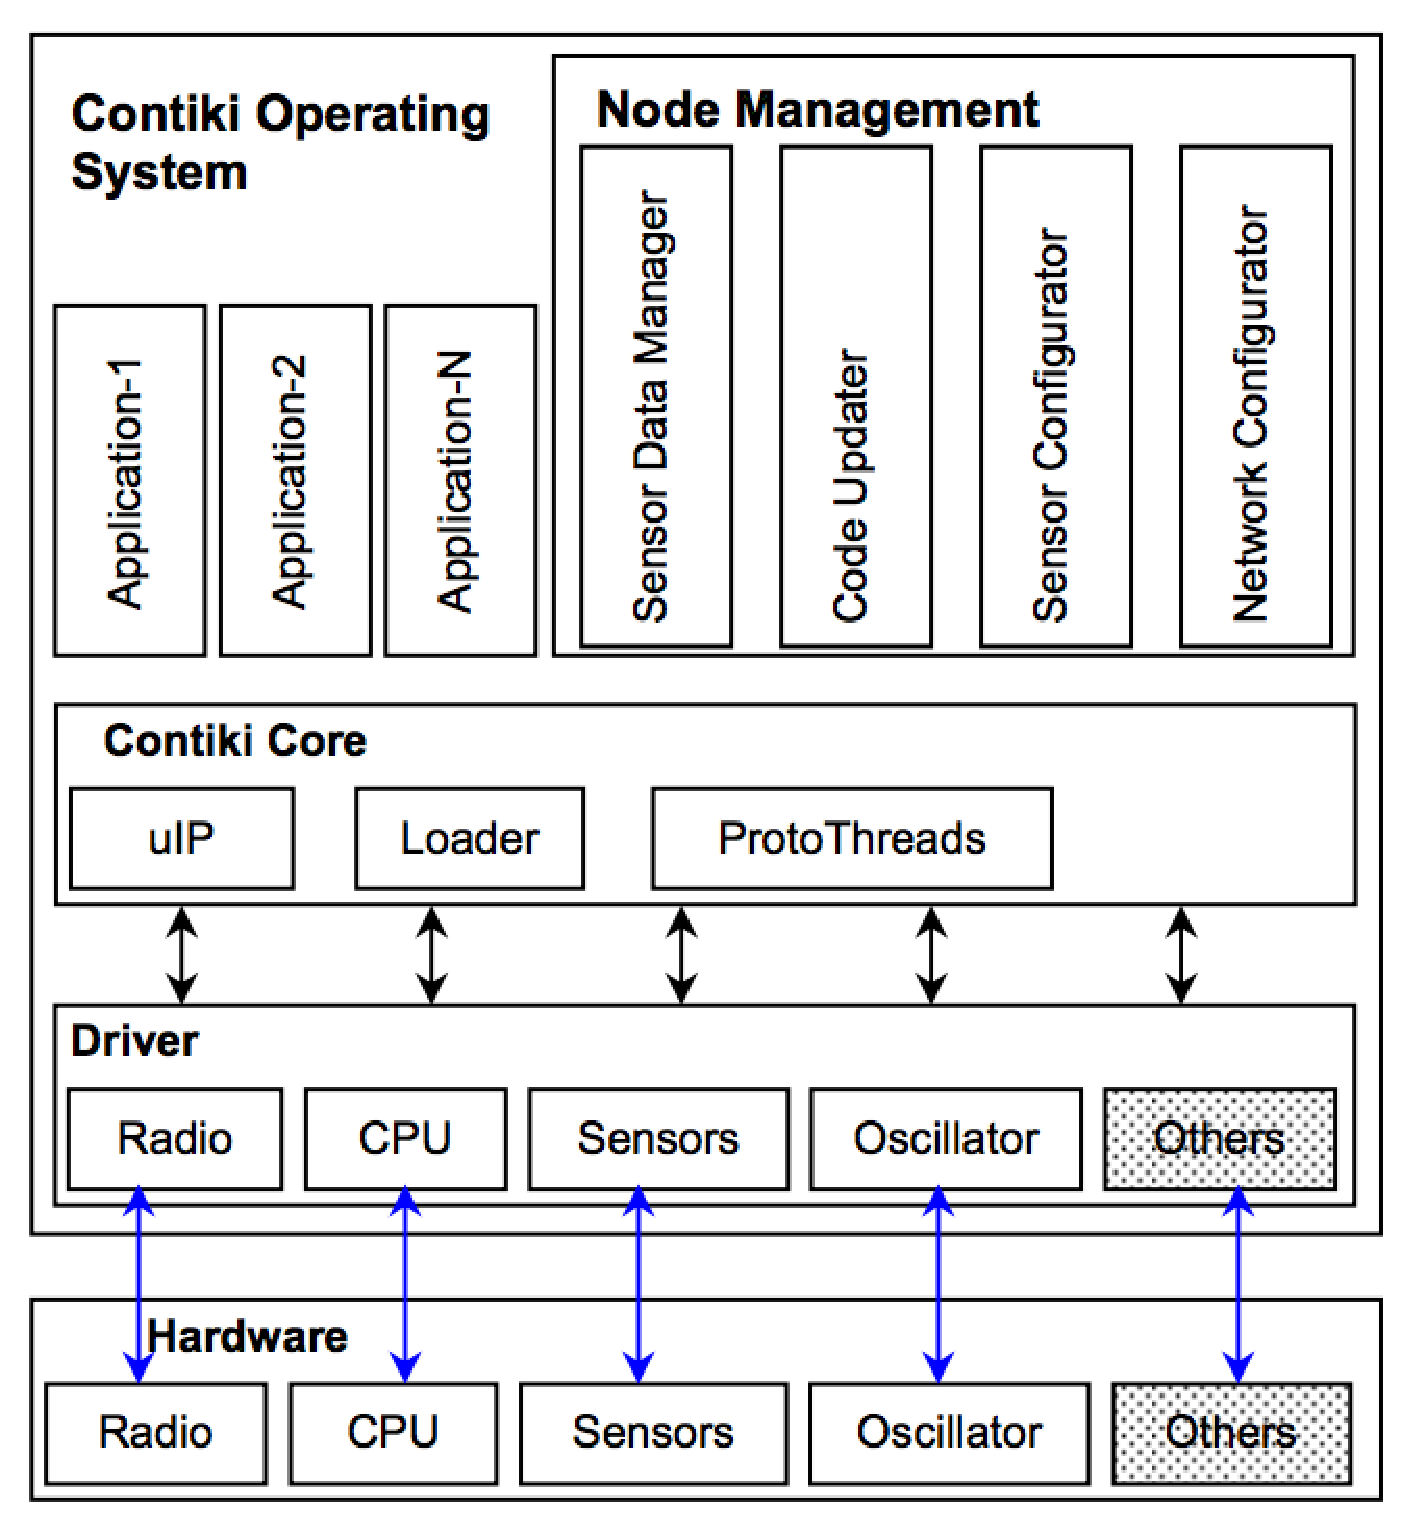
\includegraphics[width=80mm]{./images/system_conf_of_contiki.eps}
 \end{center}
 \caption{Contiki アーキテクチャ}
 \label{fig:system_conf_of_contiki}
\end{figure}




\section{スレッドモデル}\label{sec:threads_model}
%スレッドモデルを図 5 に示す.
スレッドモデルは図\ref{fig:threads_model}に示されるように,
複数のスレッドから構成され,
各スレッドはそれぞれ独立に実行ストリームを持っており,
低い優先度のスレッドは高い優先度のスレッドにプリエンプションされるという特徴を持つ.
スレッドモデルではユーザはあたかもCPUを占有しているかのように
一連の処理をひとつのスレッドとして記述することができるため,
プログラムが書きやすい.
またプリエンプションを行うことも想定しているため,
%ジョブの実行を設定された時間通りに作動させる,
リアルタイム処理をサポートすることができる.
本節では,スレッドモデルの例として,
MANTIS OSとNano-RKを紹介し,
その特徴について考察する.



\begin{figure}[htbp]
 \begin{center}
  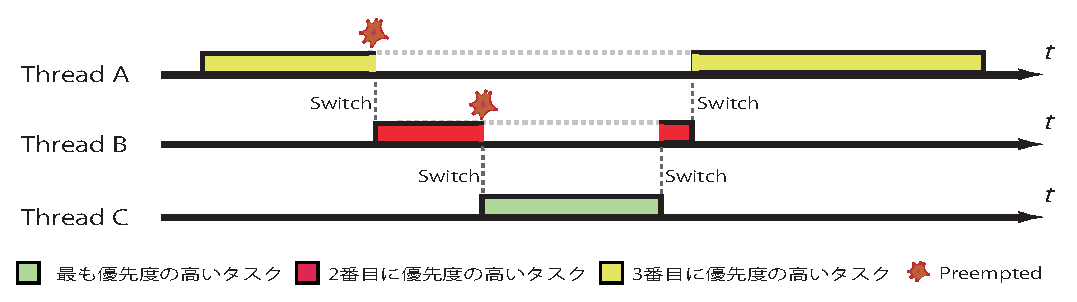
\includegraphics[width=140mm]{./images/threads_model.eps}
 \end{center}
 \caption{スレッドモデル}
 \label{fig:threads_model}
\end{figure}



%\subsection{MANTIS OS: An Embedded Multithreaded Operating System for Wireless Micro Sensor Platforms}
\subsection{MANTIS OS}
MANTIS OS\cite{Bhatti:2005:MOE:1160162.1160178}はLinuxやFreeBSDなどで
用いられているスレッドと同様の機能をセンサノード上で
実現したスレッドモデルのオペレーティングシステムである.
開発者はLinuxやFreeBSDなどで用いられているソフトウェアを
大きな変更なくMANTIS OS上に移植することができる.
また,MANTIS OS上の1つのスレッドとして
TinyOS\cite{Hill:2000:SAD:356989.356998}\cite{Levis04tinyos:an}を
実装することも可能であり\cite{Trumpler06asystematic},
さまざまなソフトウェアリソースをMANTIS OS上で動作可能であることも特徴的である.
MANTIS OSはC言語で実装されており,
アプリケーション開発者もC言語を用いて開発を行うことが可能である.
図\ref{fig:system_conf_of_mantis}はMANTIS OSのアーキテクチャである.

%The MultimodAl system for NeTworks of In-situ wireless Sensors (MANTIS) provides 
%a new multithreaded operating system for WSNs.
%MANTIS is a lightweight and energy efficient operating system. 
%It has a footprint of 500 bytes, 
%which includes kernel, scheduler, and network stack. 
%The MANTIS Operating System (MOS) key feature is that 
%it is portable across multiple platforms, 
%i.e., we can test MOS applications on a PDA or a PC [28].
%Afterwards, the application can be ported to the sensor node.
%MOS also supports remote management of sensor nodes through dynamic programming. 
%MOS is written in C and it supports application development in C.
%The following subsections discuss the design features of MOS in more detail

\begin{figure}[htbp]
 \begin{center}
  \includegraphics[width=80mm]{./images/system_conf_of_mantis.eps}
 \end{center}
 \caption{MANTIS OS アーキテクチャ}
 \label{fig:system_conf_of_mantis}
\end{figure}




%\subsection{Nano-RK: an Energy-aware Resource-centric RTOS for Sensor Networks}
\subsection{Nano-RK}
Nano-RK\cite{Eswaran:2005:NER:1106608.1106672}は,
無線センサネットワークにおけるマルチタスク処理機能を備えた
リアルタイムオペレーティングシステムであり,
%Nano-RK [31] is a fixed, preemptive multitasking real-time OS for WSNs. 
%Nano-RKを設計することで,
リソースの使用が制限された無線センサネットワークにおける,
マルチタスク処理や
優先度順位スケジューリング,
マルチホップネットワークのサポートを実現する.
%The design goals for Nano-RK are multitasking, support for multi-hop networking, 
%support for priority-based scheduling, 
%timeliness and schedulability, extended WSN lifetime, 
%application resource usage limits, and small footprint.
2KbitsのRAMと18KbitsのROMを使用し,
Rate Monotonic Scheduleing\cite{Liu:1973:SAM:321738.321743}と
Rate Harmonized Scheduling\cite{Rowe:2008:RSS:1475690.1475895}を利用することによって,
ハードリアルタイムアプリケーションとソフトリアルタイムアプリケーションの
両方をサポートする.
%Nano-RK uses 2 Kb of RAM and 18 Kb of ROM. Nano-RK provides support for CPU, 
%sensors, and network bandwidth reservations.
%Nano-RK supports hard and soft real-time applications 
%by the means of different real-time scheduling algorithms, 
%e.g., rate monotonic scheduling and rate harmonized scheduling [32]. 
現在動作確認がとれているセンシングプラットフォームとして,
MicaZ\cite{Hill:2002:MWP:623308.624560}と
FireFly\cite{Rowe_firefly:a}
が挙げられる.
Nano-RKのアーキテクチャは図\ref{fig:system_conf_of_nrk}のとおりである.
%Nano-RK provides networking support through socket-like abstraction. 
%Nano-RK supports FireFly [33] and MicaZ sensing platforms. 

\begin{figure}[htbp]
 \begin{center}
  \includegraphics[width=100mm]{./images/system_conf_of_nrk.eps}
 \end{center}
 \caption{Nano-RK アーキテクチャ}
 \label{fig:system_conf_of_nrk}
\end{figure}






\section{イベントモデルとスレッドモデルの比較}\label{sec:comparison_between_event_and_threads}
表\ref{tab:merit_and_demerit}にイベントモデルとスレッドモデルにおける
メリットとデメリットを示す.
既に述べたように,
イベントモデルではプリエンプションされることを前提としていないため,
実行ストリームがひとつで実現され,
ローカル変数の領域がそれぞれのタスクで共有することができるようになることから,
%省資源で低オーバヘッドな
消費電力の少ないシステムを構築することが可能になる.
しかしながら,イベントモデルではユーザが一連の処理を細かい処理に分割しなければならないため,
アプリケーションの開発が困難になってしまい,
%アプリケーション開発時に開発者がプログラムを書き辛いという問題が発生する.
リアルタイム処理のサポートもできない.
%さらに,イベントモデルではタスクのプリエンプションをしないことを前提に設計されているので
%ハードリアルタイム処理のサポートができない.


イベントモデルに対して,
スレッドモデルでは複数のスレッドがそれぞれ独立に実行ストリームを保持しているため,
プリエンプションを可能とする.
結果として,スレッドモデルではリアルタイム性をサポートすることができる.
また,それぞれの処理をひとつのスレッドとみなし記述をすることが可能となるため,
開発者がアプリケーションを開発することを容易にする.
しかしながら,プリエンプション時の
%オーバヘッドの大きいことや必要とされる資源が多いこと,
電力の消費が激しいことや,
スレッド間の共有資源へのアクセス制御が必要となるために
安全性が損なわれるなどの欠点を兼ね備えている.


%本節で述べたとおり,
%
%イベント駆動モデルではタスクの中断をしないことを前提に設計されているため,
%現在のセンサネットワーク用のオペレーティングシステムでは
%省資源性かつ低オーバヘッドであることと,
%リアルタイム性のサポートはトレードオフの関係にある.



\begin{table}[htb]
  \centering
  \caption{オペレーティングシステムの比較}
  \begin{tabular}{|c||c|c|c|c|} \hline
    \backslashbox{}{} & \multicolumn{2}{|c|}{メリット} & \multicolumn{2}{|c|}{デメリット} \\ \hline \hline
    イベントモデル & \multicolumn{2}{|c|}{低消費電力} & バッチ処理の採用 & 開発が困難である \\ \hline
    %スレッドモデル & \multicolumn{2}{|c|}{リアルタイム性のサポート} & 資源の消費が大きい & 高オーバヘッド \\ \hline
    スレッドモデル & \multicolumn{2}{|c|}{リアルタイム性のサポート} & \multicolumn{2}{|c|}{高消費電力} \\ \hline
  \end{tabular}
  \label{tab:merit_and_demerit}
\end{table}





\section{まとめ}
%本章では,まず,センサネットワークの一般公衆化について述べた.次いで,公衆センサデータがを扱ったシステム設計をする際に,データ管理の時間的密度という要素を考慮すべきであることを示した.そして,センサデータが時間的特殊性を持った多次元データであることを述べ,また,それに起因するセンサデータ管理における問題を提起した.
%システムにおける地理的探索の必要性について記した.さらに,センサデータ以外のコンテンツを扱うシステムとセンサデータを扱うシステムの対比を行い,広域センサデータ管理システムにおけるデータ管理の時間的密度という概念を説明し,最後に,センサデータの時間的特殊性を取り上げた後,それに起因するセンサデータ管理におけるデータ管理の時間的密度の高さという問題を提起した.
%本章では,まず,公衆広域センサデータが多次元データであるということから,本研究の根幹を
%成す,Multidimensional Indexing(MI)という研究分野を紹介した.次に,Contents Delivery
%Network(CDN)という分散したデータセンターで多次元データを管理するネットワークという
%観点から捉え,センサデータには CDN で扱われるような特殊性が存在しないことを述べた.最後
%に,公衆広域センサデータの分散管理手法を紹介し,センサデータの時間的特殊性が考慮されてい
%ないことに言及した.


本章では,
まず,無線センサネットワークにおけるオペレーティングシステムについて導入した.
次いで,無線センサネットワークにおけるオペレーティングシステムを
イベントモデルとスレッドモデルの2つのモデルに大別し,
各モデルにおけるオペレーティングシステムの概要を述べた.
最後に,イベントモデルとスレッドモデルを比較し,
イベントモデルではタスクの中断をしないことを前提に設計されているため,
現在のセンサネットワーク用のオペレーティングシステムでは
%省資源性かつ低オーバヘッド
低消費電力であることと,
リアルタイム性のサポートはトレードオフの関係にあるということを示した.




